\documentclass[UTF8]{ctexart}
\usepackage{graphicx}
\usepackage{multirow}
\usepackage{booktabs}
\usepackage{latexsym}
\usepackage{indentfirst}
\setlength{\parindent}{2em}
\usepackage{color}
\definecolor{lbcolor}{rgb}{0.9,0.9,0.9}
\usepackage{listings}
\lstset{backgroundcolor=\color{lbcolor}}
\lstset{keywordstyle=\color[rgb]{0,0,1}}
\lstset{commentstyle=\color[rgb]{0.133,0.545,0.133}}
\lstset{stringstyle=\color[rgb]{0.627,0.126,0.941}}
\lstset{language=Matlab}
\lstset{numbers=left}
\lstset{breaklines=true}
\author{何舜成}
\date{2012011515}
\title{Image Processing Exercise 2}
\begin{document}
\maketitle
\section{问题描述}
有如下暗光拍摄图像,请使用适当的方法处理该图像,增强图像的亮度。\par
\begin{figure}[htbp]
\centerline{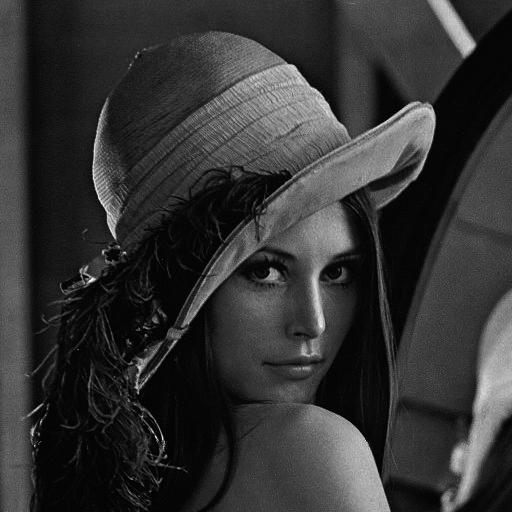
\includegraphics[width=3.5in]{lena.jpg}}
\caption[]{lena.jpg}
\end{figure}
\section{问题解答}
为了增强图像亮度,只需要对图像做逐点运算,选取一个函数$f(x)$,满足$\forall x\in[0,1], f(x)>x$,那么输出的图像的亮度得到了增强。在这次实验中,我们选取了$f(x)=\sqrt{x}$。\par
最终得到如下效果,可以看到处理后比原图更亮了。\par
\begin{figure}[htbp]
\centerline{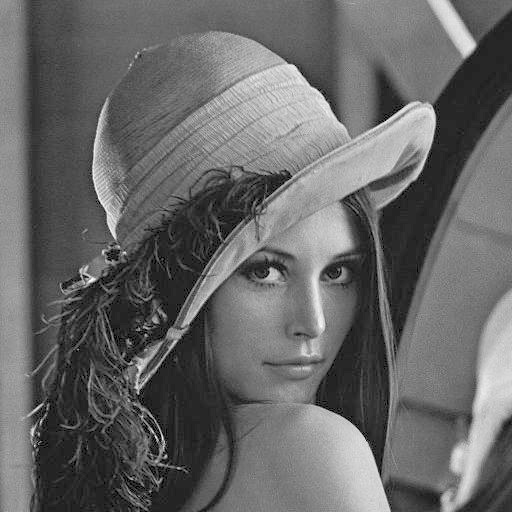
\includegraphics[width=3.5in]{lena-light.jpg}}
\caption[]{lena-light.jpg}
\end{figure}\par
程序采用OpenCV编写,版本2.4.11,开发环境Xcode 7.0.1,使用C++98标准,标准库libstdc++。
\end{document}